\chapter{Pendahuluan}
\label{chap:pendahuluan}

\section{Latar Belakang}
\label{sec:latar belakang}

Seiring dengan perkembangan zaman, perkembangan internet di Indonesia sudah semakin maju.  Banyak orang sudah menggunakan fasilitas internet untuk berbagai macam kebutuhan. Contoh dari penggunaan internet adalah untuk mencari informasi, email, bermain jejaring sosial online, Internet Banking, online shop, dan lain lain. Menurut Kemkoinfo \footnote{bint005,Pengguna Internet di Indonesia Capai 82 Juta, http://kominfo.go.id/index.php/content/detail/3980/Kemkominfo\%3A+Pengguna+Internet+di+Indonesia+Capai+82+Juta/0/berita_satker, diakses 9 September 2014, jam 10.42 WIB} pengguna internet di Indonesia capai 82 Juta orang, delapan puluh persen diantaranya adalah remaja. Hal ini menunjukkan bahwa internet sudah tidak asing lagi untuk masyarakat di Indonesia ini. Sebagai informasi tambahan bahwa pengguna internet di Indonesia 95 persennya digunakan untuk social media atau jejaring social online. Salah satu social media yang banyak digunakan adalah Twitter. Twitter adalah salah satu layanan jejaring sosial online yang memungkinkan pengguna memposting pesan berbasis teks hingga 140 karakter. Terdapat banyak keunggulan Twitter dibandingkan social media yang lain yaitu alat komunikasi yang cepat tanggap, extensible messaging platform degnan API terbuka, jangkauan yang luas kita dapat memfollow siapa saja, dapat mengetahui secara cepat trend yang sedang terjadi, tidak memakan kuota yang banyak karena berbasis teks, dan lain lain. 

%Twitter adalah salah satu layanan jejaring sosial online yang memungkinkan pengguna memposting pesan berbasis teks hingga 140 karakter. Pengguna Twitter menyebutnya sebagai \textit{tweet}. \textit{Tweet} ini akan meneruskan pesan singkat yang ditujukan ke semua \textit{follower} suatu akun\footnote{Dusty Reagan, \textit{Twitter Application Development For Dummies}, Wiley, 2010, page 7}.\textit{Follow} adalah salah satu istilah dalam Twitter yang bertujuan untuk mengikuti aktivitas \textit{tweet} suatu akun. Sedangkan cara seseorang untuk dapat memberi rujukan kepada akun Twitter yang lainnya adalah dengan cara \textit{reply} atau lebih dikenal dengan nama \textit{mention}\footnote{Dusty Reagan, \textit{Twitter Application Development For Dummies}, Wiley, 2010, page 9}. Sebagai contoh, diketahui akun bernama @kviniink mem-\textit{follow} @infobdg untuk mengetahui perkembangan apa saja yang tejadi di kota Bandung. Lalu akun @kviniink ingin bertanya tentang info mall yang ramai di Bandung, maka akun @kviniink membuat \textit{mention tweet} yang berisikan "@infobdg Halo saya ingin bertanya apa saja mall yang sedang ramai di Bandung yah?".

Hal lain yang banyak digunakan oleh kebanyakan orang di dunia adalah transportasi publik, bukan hanya di Indonesia saja transportasi publik ini sudah banyak digunakan di luar negeri. Menurut data yang ada, angkutan umum di Kota Bandung pada tahun 2013 sudah lebih dari 12000 unit kendaraan. Keuntungan memakai transportasi publik sudah banyak dirasakan di seluruh dunia yaitu untuk mengatasi kemacetan dan mengurangi pemanasan global. Seiring dengan perkembangan teknologi, menaiki transportasi publik menjadi semakin mudah. KIRI adalah sebuah situs atau \textit{website} yang memberi panduan tentang jalur transportasi publik. Dengan adanya KIRI di Indonesia terutama di daerah Bandung, masyarakat dapat naik transportasi publik tanpa harus mengetahui terlebih dahulu kendaraan yang harus dinaikinya. 

KIRI dan Twitter menyediakan API-nya masing-masing. KIRI API adalah aplikasi pihak ketiga yang memungkinkan \textit{programmer} mendapatkan data tentang info jalur transportasi publik. Twitter API adalah aplikasi pihak ketiga yang memungkinkan \textit{programmer} melakukan manipulasi dan pengolahan data di Twitter. Dengan memanfaatkan KIRI API dan Twitter API peneliti akan membangun sebuah perangkat lunak yang dapat memudahkan pengguna dalam mencari jalur transportasi publik. Sebuah applikasi yang menggabungkan jejaring sosial online Twitter dengan KIRI API. Program yang dibuat akan bersifat real time sehingga jika seseorang melakukan mention kepada bot pencari jalur maka bot akan menangkapnya dan membalas mention tersebut berupa jalur yang harus ditempuh.% Jadi pengguna bisa melakukan \textit{tweet} kepada Twitter bot yang dibuat dengan format tertentu yang berisikan tempat asal dan tempat yang akan dituju. Lalu pengguna akan menerima balasan tweet berupa rute jalan yang harus ditempuhnya secara real time.

% Contoh dari jalannya program adalah
%\begin{itemize}
	%\item Akun bernama @kviniink melakukan \textit{mention} kepada @kiriupdate untuk bertanya jalur transportasi publik,"@kiriupdate \#find bip to ip".
	%\item Twitter bot @kiriupdate akan mendengarkan mention dari akun @kviniink lalu mention tersebut akan diolah oleh server dan akan melakukan reply kepada akun @kviniink
	%\begin{enumerate}
		%\item "@kviniink istana plaza to bandung indah plaza",
		%\item "@kviniink Walk about 135 meter from your starting point to Jalan Aceh." ,
		%\item "@kviniink Take angkot Ciroyom - Antapani at Jalan Aceh, and alight at Jalan Pajajaran about 3.6 kilometer later.",
		%\item "@kviniink Walk about 93 meter from Jalan Pajajaran to your destination.".
	%\end{enumerate}
%\end{itemize}

%\begin{figure}[hp]
	%\centering
		%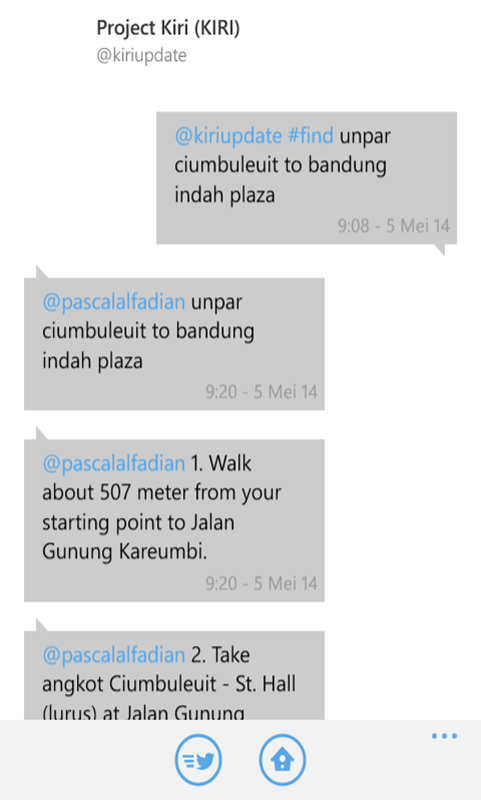
\includegraphics[width=0.50\textwidth]{C:/Users/Kvin/git/Skripsi/doc/DokumenSkripsi/Gambar/contohpercakapan.png}
	%\label{fig:contohpercakapan}
%\end{figure}
%Karena keterbatasan 140 karakter maka tweet akan dipecah sesuai dengan instruksi yang dikirimkan dari KIRI API.

\section{Rumusan Masalah}
Mengacu kepada deskripsi yang diberikan, maka rumusan masalah pada penelitian ini adalah:
\begin{itemize}
	\item Bagaimana membuat \textit{Twitter bot} untuk mencari jalur transportasi publik?
	\item Bagaimana membuat \textit{Twitter bot} untuk dapat merespon secara real time?
	\item Bagaimana memformat petunjuk rute perjalanan dalam keterbatasan tweet 140 karakter?
\end{itemize}

\section{Tujuan}
Tujuan dari penelitian ini adalah:
\begin{itemize}
	\item Membuat aplikasi \textit{Twitter bot} untuk mencari jalur transportasi publik.
	\item Membuat aplikasi \textit{Twitter bot} yang bekerja secara \textit{real time}.
	\item Membuat algoritma untuk memecah instruksi dari KIRI API dan mengubahnya ke dalam bentuk tweet.
\end{itemize}

\section{Batasan Masalah}
Pada pembuatan perangkat lunak ini, masalah-masalah yang ada akan dibatasi menjadi:
\begin{itemize}
	\item Input hanya mencakup Kota Bandung saja.
	\item Applikasi tidak menangani input yang tidak valid.
\end{itemize}

\section{Metode Penelitian}
Pada perangkat lunak yang dibuat ini digunakan beberapa metode dalam penyelesaian masalah yang menjadi topik pada penelitian ini, antara lain:
\begin{enumerate}
	\item Melakukan studi literatur terhadap KIRI API dan Twitter API
	%\begin{itemize}
		%\item KIRI API,
		%\item REST API Twitter (https://dev.twitter.com/docs/api/1.1),
		%\item Streaming API Twitter (https://dev.twitter.com/docs/api/streaming).
	%\end{itemize}
	%\item Mempelajari pembuatan server dalam bahasa Java.
	%\item Membuat TwitterBot sederhana
	%\item Melakukan analisis terhadap teori-teori yang sudah dipelajari, guna membangun perangkat lunak yang dimaksud.
	%\item Melakukan pengujian terhadap system yang sudah dibangun
	\item Menganalisa masalah
	\item Merancang perangkat lunak
	\item Mengimplementasi perangkat lunak
	\item Melakukan pengujian terhadap perangkat lunak
	\item Membuat suatu kesimpulan
\end{enumerate}.
